\documentclass[11pt, oneside]{article}   	% use "amsart" instead of "article" for AMSLaTeX format
\usepackage{geometry}                		% See geometry.pdf to learn the layout options. There are lots.
\geometry{letterpaper}                   		% ... or a4paper or a5paper or ... 
%\geometry{landscape}                		% Activate for for rotated page geometry
%\usepackage[parfill]{parskip}    		% Activate to begin paragraphs with an empty line rather than an indent
\usepackage{graphicx}				% Use pdf, png, jpg, or eps� with pdflatex; use eps in DVI mode
								% TeX will automatically convert eps --> pdf in pdflatex		
\usepackage{amssymb}
\usepackage{amsmath}
\usepackage{parskip}
\usepackage{color}

\title{Examples for Stokes theorem}
%\author{The Author}
%\section{}
% \subsection*{R code}
\date{}							% Activate to display a given date or no date

\graphicspath{{/Users/telliott_admin/Dropbox/Tex/png/}}

% \begin{center} 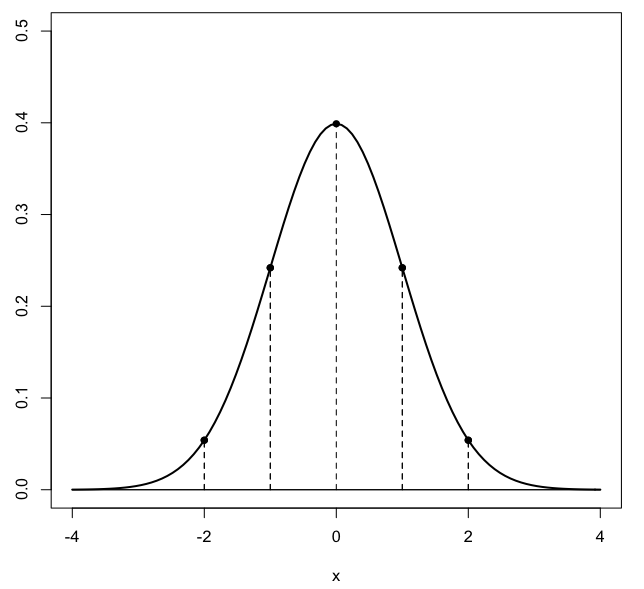
\includegraphics [scale=0.4] {gauss3.png} \end{center}
% \begin{bmatrix} a  &  b \\ c  &  d \end{bmatrix}
% \bigg |_

\begin{document}
\maketitle
\large
%\noindent
State the theorem:
\[ \oint_C \mathbf{F} \cdot \mathbf{r} = \iint_R (\nabla \times \mathbf{F}) \cdot \hat{\mathbf{n}} \ dS \]
By the usual reasoning, since $d\mathbf{r} = \ <dx,dy,dz>$, the left-hand side is
\[ P \ dx + Q \ dy + R \ dz \]
Now, suppose we have 
\[ \mathbf{F} = \ <z,x,y> \]
and $C$ is the unit circle in the $xy$-plane,
then 
\[ P \ dx + Q \ dy + R \ dz = \oint_C  z \ dx + x \ dy + y \ dz =   \oint_C x \ dy \]
Parameterize
\[ C =
\left\{
	\begin{array}{l}
		x  = \cos t  \\
		y  = \sin t
	\end{array}
\right.
\]
we have
\[ \oint_C x \ dy = \int_0^{2\pi} \ \cos t \ \cos t \ dt \]
\[ = \frac{1}{2}(t + \frac{1}{2} \sin t) \ \bigg |_0^{2\pi} = \pi \]
For the surface, we can use anything that passes through $C$, let's use the paraboloid for fun.
\[ z = 1 - x^2 - y^2 \]
We need the curl of $\mathbf{F} = \ <z,x,y> $
\[ \nabla \times \mathbf{F} = \ < 1,1,1> \]
We need
\[ \hat{\mathbf{n}} \ dS = \ <-f_x,-f_y,1> \ dx \ dy =  \ <2x,2y,1> \ dx \ dy \]
so
\[ \iint_R (\nabla \times \mathbf{F}) \cdot \hat{\mathbf{n}} \ dS =  \iint_R \ 2x + 2y + 1 \ dx \ dy \]
Again, $C$ is the unit circle in the $xy$-plane.  To save effort, we can notice that 
\[ \int x \ dx = \overline{x} \]
What is the \emph{average} value of $x$ over the unit circle?  It is just equal to $0$.  The same thing is true for the second integrand (reverse the order of integration).  So we have just
\[ \iint_R \  1 \ dx \ dy = \pi \]
which matches what we had above.

Suppose we hadn't seen this.  We could just do
\[ \int_{x=-1}^{1} \int_{y=-\sqrt{1-x^2}}^{\sqrt{1-x^2}} \ x \ dy \ dx \]
\[ = \int_{x=-1}^{1} 2 \sqrt{1-x^2} \ x \ dy \ dx \]
\[ = - \frac{2}{3} \ (1-x^2)^{3/2} \ \bigg |_{-1}^1 \]
At both bounds, $1-x^2 = 0$, so the whole thing is $0$.

\end{document}  